\section{Auswertung}
\label{sec:Auswertung}
    Die gemessenen Werte sind in Tabelle ??? dargestellt.
    \begin{figure}
        \centering
        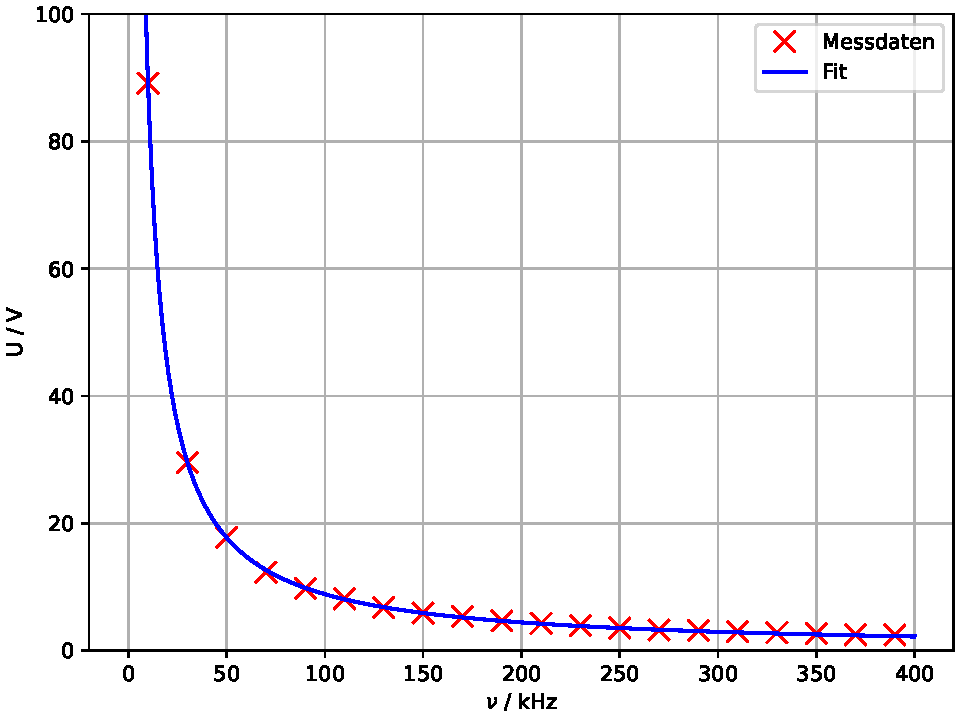
\includegraphics[height= 5cm]{build/plota.pdf}
        \caption{Die Temperatur in Abhängigkeit der Zeit der beiden Reservoire.}
        \label{abb:Fit_Temperatur}
    \end{figure}
    In Abbildung \ref{abb:Fit_Temperatur} ist die Temperatur aufgetragen gegen die Zeit.
    \subsection{Ausgleichsrechnung}
    Für die Ausgleichsrechnung wurde die Funktion
    \begin{equation}
        T(t) = at^2+bt+c
        \label{eq:Ausgleich}
    \end{equation}
    gewählt.
    Mittels Python werden folgende Werte errechnet
    \begin{align*}
        a_1 &= \SI{-4.6(1.1)e-6}{\degreeCelsius\per\square\second}
        & a_2 &= \SI{10.4(1.9)e-6}{\degreeCelsius\per\square\second}\\
        b_1 &= \SI{3.2(0.2)e-2}{\degreeCelsius\per\second}
        & b_2 &=\SI{3.3(0.3)e-2}{\degreeCelsius\per\second}\\
        c_1 &=\SI{18.0(0.4)}{\degreeCelsius}
        & c_2 &=\SI{25.6(0.7)}{\degreeCelsius}
    \end{align*}
    wobei die Werte mit dem Index 1 den Verlauf der blauen Kurve beschreiben
    und die Werte mit dem Index 2 den der orangenen Kurve beschreiben.

    \subsection{Berechnung der Differentialquotienten}
    Die Differentialquotienen $\sfrac{dT_i}{dt}$ berechnen sich durch einsetzen von $t$ in die Ableitung
    von \autoref{eq:Ausgleich}, $T'(t) = 2At+B$.
    \begin{table}[H]
      \centering
      \begin{tabular}{
        S[table-format=4.0]
        S[table-format=2.3]
        S[table-format=2.3]
        S[table-format=3.0]
      }
        \toprule
        {$t\left[\unit{s}\right]$} & {$\frac{dT_1}{dt}\left[\unit{\frac{°C}{s}}\right]$} & {$\frac{dT_2}{dt}\left[\unit{\frac{°C}{s}}\right]$} & {$N\,\left[\unit{W}\right]$}\\
        \midrule
        300 &  {$0,029 \pm 0,002$}  & {$-0,027 \pm 0,004$} & 200\\
        600 &  {$0,026 \pm 0,003$}  & {$-0,021 \pm 0,005$} & 206\\
        900 &  {$0,023 \pm 0,004$}  & {$-0,015 \pm 0,006$} & 210\\
        1200 & {$0,021 \pm 0,004$}  & {$-0,008 \pm 0,007$} & 205\\
        \bottomrule
    \end{tabular}
      \label{tab:Diffquot}
    \caption{Differentialquotienten für vier Zeiten der zwei Messreihen.}
    \end{table}
    Die errechneten Werte sind in \autoref{tab:Diffquot} dargestellt.

    \subsection{Berechnung der Güteziffer}
    Die ideale Güterziffer lässt sich über ??? berechnen.
    Die reale Güteziffer wird mit ??? berechnent.
    Hierbei gilt $m_1 = 3\,\unit{kg}$ und $c_w = \SI{4200}{\joule\per\kg\per\kelvin}$.
    Die Wärmekapazität der Kupferschlange und der Reservoire ist $m_\text{k} c_\text{k} = \SI{750}{\joule\per\kelvin}$.
    Die Güteziffern sind in \autoref{tab:Guete} aufgeführt.
    \begin{table}
  \centering
  \begin{tabular}{
    S[table-format=4.0]
    S[table-format=2.3]
    S[table-format=2.3]
    S[table-format=2.3]
    S[table-format=2.3]
    S[table-format=2.3]
  }
    \toprule
    {$t\left[\unit{s}\right]$} & {$v_{\text{ideal}}$} & {$v_{\text{real}}$ für $T_1$} & {$v_{\text{real}}$ für $T_2$}
    & {$\Delta v_1$} & {$\Delta v_2$}\\
    \midrule
    300 & 2.87  & {$1,9 \pm 0,1$} & {$-1,8 \pm 0,3$} & 0.94 & 1.07\\
    600 & 1.34  & {$1,7 \pm 0,2$} & {$-1,4 \pm 0,3$} & 0.34 & 0.02\\
    900 & 1.09  & {$1,5 \pm 0,3$} & {$-1,0 \pm 0,4$} & 0.37 & 0.14\\
    1200 & 1.02 & {$1,4 \pm 0,3$} & {$-0,5 \pm 0,5$} & 0.35 & 0.50\\
    \bottomrule
\end{tabular}
\caption{Ideale und reale Güteziffer für vier Zeiten und deren Abweichung}
        \label{tab:Guete}
\end{table}

    \subsection{Die Verdampfungswärme L}
    Die Verdampfungswärme des Transportgases kann aus seiner Dampfdruckkurve bestimmt werden.
    Die Dampfdruck-Kurve wird aus den Messwerten $T_1$ und $p_\text{b}$ gewonnen.
    Dafür wird der Logarithmus der Drucks $p_b$ gegen die reziproke absolute Temperatur $T_1$ aufgetragen.
    \begin{figure}[H]
        \centering
        \includegraphics[height=7cm]{build/Verdampfungswärme.pdf}
        \caption{Die Messwerte des warmen Reservoirs aufgetragen als
        der Logarithmus der Drucks $p_b$ gegen die reziproke absolute Temperatur
        $T_1$ mit der Ausgleichsgeraden. $p_0 = 1001mbar$}
    \end{figure}
    Die Gleichung zur Bestimmung von $L$ und dem damit einhergehenden Fit ist
    \begin{equation}
        \ln(p) = - \frac{L}{R} \cdot \frac{1}{T}
        \Rightarrow y = m \cdot x + b \, \text{.}
    \end{equation}
    Nummeric Python berechnet $m = \SI{2726 \pm 179}{\kelvin}$ und $b = 4.1 \pm 0.6$.
    Damit ergibt sich mit $L = -a \cdot R$, wobei $R$ die Universelle Gaskonstante mit dem Wert
    $R = \SI{8.314}{\joule\per\mole\per\kelvin}$ \cite{Gaskonstante},
    \begin{equation*}
        L = \SI{2.27(0.15)e+4}{\joule\per\mol} \, \text{.}
    \end{equation*}
